\newcommand{\nom}{Porte conteneur}
\newcommand{\sequence}{03}
\newcommand{\num}{04}
\newcommand{\type}{TD}
\newcommand{\descrip}{Résolution d'un problème en utilisant des méthodes algorithmiques}
\newcommand{\competences}{Alt-C3: Concevoir un algorithme répondant à un problème précisément posé}
\documentclass[10pt,a4paper]{article}
  \usepackage[french]{babel}
  \usepackage[utf8]{inputenc}
  \usepackage[T1]{fontenc}
  \usepackage{xcolor}
  \usepackage[]{graphicx}
  \usepackage{makeidx}
  \usepackage{textcomp}
  \usepackage{amsmath}
  \usepackage{amssymb}
  \usepackage{stmaryrd}
  \usepackage{fancyhdr}
  \usepackage{lettrine}
  \usepackage{calc}
  \usepackage{boxedminipage}
  \usepackage[french,onelanguage, boxruled,linesnumbered]{algorithm2e}
  \usepackage[colorlinks=false,pdftex]{hyperref}
  \usepackage{minted}
  \usepackage{url}
  \usepackage[locale=FR]{siunitx}
  \usepackage{multicol}
  \usepackage{tikz}
  \makeindex

  %\graphicspath{{../Images/}}

%  \renewcommand\listingscaption{Programme}

  %\renewcommand{\thechapter}{\Alph{chapter}}
  \renewcommand{\thesection}{\Roman{section}}
  %\newcommand{\inter}{\vspace{0.5cm}%
  %\noindent }
  %\newcommand{\unite}{\ \textrm}
  \newcommand{\ud}{\mathrm{d}}
  \newcommand{\vect}{\overrightarrow}
  %\newcommand{\ch}{\mathrm{ch}} % cosinus hyperbolique
  %\newcommand{\sh}{\mathrm{sh}} % sinus hyperbolique

  \textwidth 160mm
  \textheight 250mm
  \hoffset=-1.70cm
  \voffset=-1.5cm
  \parindent=0cm

  \pagestyle{fancy}
  \fancyhead[L]{\bfseries {\large PTSI -- Dorian}}
  \fancyhead[C]{\bfseries{{\type} \no \numero}}
  \fancyhead[R]{\bfseries{\large Informatique}}
  \fancyfoot[C]{\thepage}
  \fancyfoot[L]{\footnotesize R. Costadoat, C. Darreye}
  \fancyfoot[R]{\small \today}
  
  \definecolor{bg}{rgb}{0.9,0.9,0.9}
  
  
  % macro Juliette
  
\usepackage{comment}   
\usepackage{amsthm}  
\theoremstyle{definition}
\newtheorem{exercice}{Exercice}
\newtheorem*{rappel}{Rappel}
\newtheorem*{remark}{Remarque}
\newtheorem*{defn}{Définition}
\newtheorem*{ppe}{Propriété}
\newtheorem{solution}{Solution}

\newcounter{num_quest} \setcounter{num_quest}{0}
\newcounter{num_rep} \setcounter{num_rep}{0}
\newcounter{num_cor} \setcounter{num_cor}{0}

\newcommand{\question}[1]{\refstepcounter{num_quest}\par
~\ \\ \parbox[t][][t]{0.15\linewidth}{\textbf{Question \arabic{num_quest}}}\parbox[t][][t]{0.85\linewidth}{#1\label{q\the\value{num_quest}}}\par
~\ \\}

\newcommand{\reponse}[4][1]
{\noindent
\rule{\linewidth}{.5pt}\\
\textbf{Question\ifthenelse{#1>1}{s}{} \multido{}{#1}{%
\refstepcounter{num_rep}\ref{q\the\value{num_rep}} }:} ~\ \\
\ifdef{\public}{#3 ~\ \\ \feuilleDR{#2}}{#4}
}

\newcommand{\cor}
{\refstepcounter{num_cor}
\noindent
\rule{\linewidth}{.5pt}
\textbf{Question \arabic{num_cor}:} \\
}


\usepackage{enumitem}

\setenumerate[1]{align=left,label=\arabic*}
\setenumerate[2]{before=\stepcounter{enumi},label*=.\arabic*,leftmargin=1.2em,align=left}


\ifdef{\public}{\excludecomment{solution}}


\begin{document}

\begin{center}
{\Large\bf {\type} \no {\numero}}
\end{center}

\SetKw{KwFrom}{de} 

\begin{boxedminipage}{.9\textwidth} 
\begin{itemize}
 \item Faire tous les exercices dans un même fichier {NomPrenom.py} à sauvegarder,
 \item mettre en commentaire l'exercice et la question traités (ex: \# Exercice 1),
 \item ne pas oublier pas de commenter ce qui est fait dans votre code (ex: \# Je crée une fonction pour calculer la racine d'un nombre),
 \item il est possible de demander un déblocage pour une question marquée *, mais celle-ci sera notée 0,
 \item il faut vérifier avant de partir que le code peut s'exécuter et qu'il affiche les résultats que vous attendez.
\end{itemize}
\end{boxedminipage}




\section*{Exercice 1 : Longueur de ligne brisée et lecture de données dans un fichier}
Le tableau suivant donne les coordonnées d'un point $M(t)$ (abscisse $x(t)$ et ordonnée $y(t)$) en divers instants $t$ :
\begin{center}
\begin{tabular}{|c||c|c|c|c|c|}
\hline
$t$ & $0.1$ & $0.2$ & $0.3$ & $0.4$ & $0.5$ \\
\hline
$x(t)$ & 1 & 0 & $-1$ & 0 & 1 \\
\hline
$y(t)$ & 0 & 1 & 0 & $-1$ & 0 \\
\hline
\end{tabular}
\end{center}
\begin{enumerate}
\item * Définir deux listes \texttt{LX} et \texttt{LY} contenant les abscisses et les ordonnées du point $M(t)$ aux divers instants~$t$.
\item Représenter les points aux divers instants $t$ ainsi que la ligne polygonale joignant ces points. \\
On utilisera \texttt{plot} et \texttt{show} du module \texttt{matplotlib.pyplot}.
\item Calculer et afficher la longueur de cette ligne polygonale.
\end{enumerate}
Les coordonnées du point $M(t)$ sont maintenant stockées dans un fichier nommé num-points.csv situé dans le répertoire /home/eleve/ressources/PTSI. Chaque ligne de ce fichier est constituée des données "$(t, x(t),y(t))$" associées à un point $M(t)$. Le séparateur de colonnes est ici ','.
\begin{enumerate}
\setcounter{enumi}{3}
\item * A partir de ce fichier, définir trois listes de flottants \texttt{LT}, \texttt{LX} et \texttt{LY} contenant les instants $t$, les abscisses et les ordonnées du point $M(t)$.
\item Vérifier que la liste \texttt{LT} est bien ordonnée selon ses valeurs croissantes.
%\item Représenter les points aux divers instants $t$ ainsi que la ligne polygonale joignant ces points.
\item Calculer et afficher la longueur de cette ligne polygonale.
\item Afficher la vitesse moyenne sur l'ensemble du parcours.
\end{enumerate}




\section*{Exercice 2}
La suite $(K_n)_{n\in \mathbb{N}}$ d'entiers naturels est définie par :
\begin{itemize}
\item $K_0=1$
\item $\forall n\in \mathbb{N}^*,~K_n=\sum\limits_{i=0}^{n-1}K_iK_{n-1-i}$
\end{itemize}
\begin{enumerate}
\item * \'Ecrire une fonction récursive \texttt{K} d'argument un entier $n$ et renvoyant $K_n$.
\item Calculer et afficher \texttt{K(2)}, \texttt{K(5)}, \texttt{K(10)} et \texttt{K(15)}. Que pensez-vous de l'efficacité de la fonction \texttt{K} ? Réponse en commentaire.
\item * \'Ecrire une fonction \texttt{fact} \textbf{(non récursive)} qui prend comme argument un entier $n$ positif et qui renvoie la valeur de la factorielle : $n!$.
\item \'Ecrire une fonction \texttt{LK} non récursive d'argument un entier $n$ et renvoyant le nombre $L_n$ donné par 
$$L_n=\frac{1}{n+1}\binom{2n}{n}.$$
Rappel : $\binom{n}{k}=\dfrac{n!}{k!(n-k)!}$
%\textit{On pourra utiliser} \texttt{comb} \textit{qui se trouve dans la sous-bibliothèque }\texttt{scipy.misc} \textit{du langage Python.}
\item Afficher en les comparant les $10$ premières valeurs de $K_n$ et de $L_n$. 
\item Que peut-on conjecturer ? Réponse en commentaire.
%\item On admet que la conjecture précédente est vérifiée pour tout entier $n$. Après avoir exprimé $L_n$ en fonction de $L_{n-1}$, proposer une méthode permettant un calcul plus efficace de $K_n$.
\end{enumerate}




\section*{Exercice 3 : tri dans le plan}
On considère le code suivant :
\begin{center}
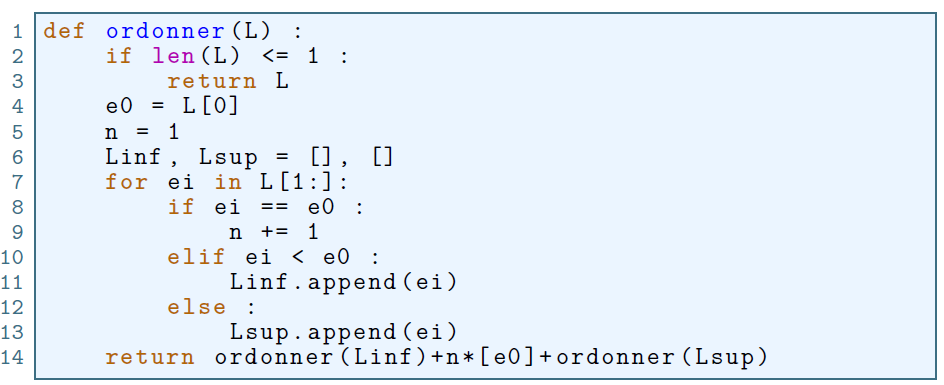
\includegraphics[scale=0.4]{ex6.png}
\end{center}
\begin{enumerate}
\item La fonction \texttt{ordonner} est une fonction de tri récursive. Pour la liste $L=[5,3,10,7,7,2]$, comptez (à la main) le nombre de fois où la fonction \texttt{ordonner} sera appelée. Réponse en commentaire.
\item Proposer et écrire une autre fonction de tri.
\item * Il n'y pas de relation d'ordre intéressante dans $\mathbb{R}^2$. On peut néanmoins construire une relation de comparaison. On dira que "$L1=[a,b]$ est inférieur à $L2=[x,y]$" si  :
\begin{center}
$a<x$ \quad ou \quad ($a=x$ et $b\leqslant y$).
\end{center}
\'Ecrire une fonction \texttt{less} de deux listes de longueur deux \texttt{L1} et \texttt{L2} qui renvoie \texttt{True} si "$L1$ est inférieur à $L2$" et \texttt{False} sinon.
\item * En s'inspirant du code définissant la fonction \texttt{ordonner}, écrire une fonction \texttt{ordonnerDansR2} qui utilise \texttt{less} et qui ordonne une liste de couples $[x,y]$ selon la relation d'ordre définie précédemment.
%\item Tester la fonction \texttt{ordonnerDansC} sur une liste de complexes dont les parties réelles et imaginaires sont des entiers tirés au hasard entre $-10$ et $10$. On pourra utiliser l'instruction \texttt{randint} du module \texttt{random}.
\item * Créer une liste \texttt{A} de flottants allant de $-\pi$ à $\pi$, avec un pas de  $\pi/100$.\\
Le nombre $\pi$ est dans la bibliothèque \texttt{math}, sous le nom \texttt{pi}.
\item * Créer la liste \texttt{L} des listes $[(20+\cos(10a))\cos(a),(20+\cos(10a))\sin(a)]$, pour $a$ parcourant la liste~\texttt{A}.\\
Les fonctions $\cos$ et $\sin$ sont dans la bibliothèque \texttt{math}.
\item Ordonner les points de \texttt{L} avec \texttt{ordonnerDansR2}. 
\item Faire tracer dans le plan le nuage de points ainsi que la ligne les reliant. On utilisera \texttt{plot} et \texttt{show} du module \texttt{matplotlib.pyplot}.% et le repère sera rendu orthonormé par \texttt{axis('equal')}.
\end{enumerate}




\section*{Exercice 4}
Dans une chaîne de caractères, on appelle "composante" une sous-chaîne correspondant à la répétition d'un même caractère, précédée et suivie par rien ou un autre caractère.

Les composantes de 'aaaaggbbbzdaa' sont : 'aaaa' suivie de, 'gg', 'bbb', 'z', 'd' et 'aa'.

%Une composante peut ensuite se coder sous la forme d'un couple \texttt{[n, c]}, où $\mathrm{n}$ désigne le nombre de répétitions du caractère $\mathrm{c}$.

\begin{enumerate}
 % \item Écrire une fonction \texttt{CP} de même argument $S$ qui renvoie une liste résultant de la mise bout-à-bout des couples codant les composantes de $S$.\\ Ainsi, \texttt{CP ('aaaaggaadaaa')} donne $\left[4, 'a', 2, 'g', 2, 'a', 1,'d', 3,'a'\right]$.
\item * Écrire une fonction \texttt{comptage} qui prend comme argument une chaîne de caractères $S$ et renvoie un dictionnaire dont chaque clé est un caractère différent de $S$ et l'élément associé à la clé est le nombre de fois que ce caractère apparaît dans $S$.\\
 Par exemple, \texttt{comptage('aaaaggbbbzdaaa')} renvoie \texttt{\{'a':7,'g':2,'b':3,'z':1,'d':1\}}. \\
 Afficher le résultat \texttt{comptage('aaaaggbbbzdaaa')}.

\item * Écrire une fonction \texttt{nbelem} dont l'argument est une chaîne de caractères $S$ et qui renvoie le nombre de caractères distincts contenus dans $S$. Par exemple, \texttt{nbelem('aaaaggbbbzdaaa')} donne 5.\\
Afficher le résultat \texttt{nbelem('aaaaggbbbzdaaa')} .
 
\item * Écrire une fonction \texttt{nbits} dont l'argument est un entier naturel $n\in\mathbb{N}^*$ et qui renvoie le plus petit entier $p\mathbb{N}^*$ tel que $n \leqslant 2^{p}$.\\
Afficher le résultat \texttt{nbits(5)}.

\item Sur l'exemple 'aaaaggbbbzdaaa', on a donc 5 lettres à coder. Il suffit pour ça de 3 bits avec le code : 'a': 000,'b': 001, 'd' :010, 'g' : 011, 'z' : 100.\\
Écrire une fonction \texttt{nbtotalbits} dont l'argument est une chaine de caractère $S$ et qui renvoie le nombre minimum de bits nécessaires pour coder les lettres de $S$.\\
Afficher le résultat \texttt{nbtotalbits('aaaaggbbbzdaaa')}.

\item Écrire une fonction \texttt{coupures} dont l'argument est une chaîne de caractères $S$, qui renvoie la liste des indices $i$ tels que $\mathrm{S}[i] \neq \mathrm{S}[i-1]$. Par exemple, coupures('aaaaggbbbzdaaa') donne $[4,6,9,10,11]$.\\
Afficher le résultat coupures('aaaaggbbbzdaaa').

\item Si $S$ est une liste composée de 45 'a' suivis de 71 'b' , quelle solution peut-on trouver pour minimiser le stockage de $S$ ? Réponse en commentaire.

\end{enumerate}

\end{document}


\begin{exercice}
\begin{enumerate}
  \item Créer une fonction parcours d'argument une liste $L=\left[a_{1}, a_{2}, \cdots, a_{n}\right]$ qui modifie cette liste en permutant $a_{k}$ et $a_{k+1}$ si $a_{k+1}<a_{k}$, pour $k$ variant de 1 à $n-1$, et qui renvoie le nombre de permutations effectuées.
\end{enumerate}
Par exemple, si $L=[5,4,1,6]$, alors parcours (L) renvoie 2 et la liste $L$ devient $L=[4,1,5,6]$.

\begin{enumerate}
  \setcounter{enumi}{2}
  \item Que peut-on dire du dernier élément d'une liste à laquelle on a déjà appliqué une fois la fonction parcours?

  \item On veut utiliser cette fonction pour trier par ordre croissant une liste selon le principe suivant: Pour une liste $L$ donnée en entrée on répète l'application de la fonction parcours jusqu'à ce que $L$ devienne invariante par cette fonction.

\end{enumerate}
Écrire une fonction tri1 qui ordonne une liste donnée en entrée selon ce principe et qui renvoie le nombre d'itérations effectuées.

\begin{enumerate}
  \setcounter{enumi}{4}
  \item Expliquer pourquoi la fonction tri1 donne bien le résultat voulu en une durée finie. Évaluer son coût de calcul dans le meilleur des cas et dans le pire des cas.

  \item Écrire une fonction tri2 comme une amélioration de la fonction tri1 en évitant les comparaisons inutiles.

\end{enumerate}
\end{exercice}



\section{Plutôt pas à prendre}


\begin{exercice}
\begin{enumerate}
  \item Pour tout entier naturel $n$, on pose $t_{n}=0+1+2+\cdots+n=\displaystyle \sum_{k=0}^{n} k$. Rappeler la valeur de $t_{n}$ en fonction de $n$. Les nombres $t_{n}$ sont appelés "nombres de type $\mathcal{T}$".

\item Construire la liste des nombres de type $\mathcal{T}$ inférieurs ou égaux à 100 .

  \item Écrire une fonction sommes de trois paramètres, deux listes $L_{1}$ et $L_{2}$ d'entiers naturels et un entier naturel $n$, renvoyant la liste strictement croissante des nombres inférieurs ou égaux à $n$ qui s'écrivent comme somme d'un élément de $L_{1}$ et d'un élément de $L_{2}$.

  \item Utiliser la fonction précédente pour obtenir la liste strictement croissante des entiers compris entre 0 et 100 qui s'écrivent comme somme de trois nombres de type $\mathcal{T}$. Que constate-t-on? Que peut-on conjecturer?

  \item Écrire une fonction decompositions d'argument un entier naturel $n$, renvoyant la liste de tous les triplets croissants de nombres de type $\mathcal{T}$ dont la somme vaut $n$. Chacun de ces triplets est une décomposition de $n$.\\
Déterminer alors le plus petit entier naturel $N$ ayant au moins 10 décompositions différentes.
  \item Évaluer le coût de calcul de la fonction decompositions.
\end{enumerate}
\end{exercice}


\begin{exercice}
\begin{enumerate}
 \item Écrire une fonction \texttt{sp} d'argument une liste $L$ qui renvoie la liste obtenue en prenant d'abord le
dernier terme de $L$, puis le premier, puis l'avant-dernier, puis le deuxième, puis l'antépénultième,
puis le troisième, \textit{etc}. (On parle de permutation en \textit{spirale}). Vérifier que \texttt{sp([1,2,3,4,5,6])} donne
bien \texttt{[6,1,5,2,4,3]}, et que \texttt{sp([1,2,3,4,5,6,7])} donne \texttt{[7,1,6,2,5,3,4]}.
\item  Vérifier que si l'on itère la fonction \texttt{sp} sur $L = [1, 2, 3, 4, 5, 6]$ on retombe sur $L$ à la sixième itération.\\
Qu'en est-il pour $L = [1, 2, 3, 4, 5, 6, 7]$ ?
\item  Écrire une fonction \texttt{periode} d'argument un entier $n$ qui renvoie le nombre minimum $p$ d'itérations de la fonction \texttt{sp} pour retomber sur la liste $[1, 2,\cdots , n]$, en partant de cette même liste.
\item  Déterminer les entiers inférieurs ou égaux à $99$ tels que \texttt{periode}$(n) = n$.
\item  À l'aide des instructions \texttt{plot} et \texttt{show} du module \texttt{matplotlib.pyplot}, faire tracer \texttt{periode}$(n)/n$ en fonction de $n$, pour $n$ compris entre $1$ et $99$. Déterminer la valeur de $n$ qui minimise \texttt{periode}$(n)/n$.
\end{enumerate}
\end{exercice}



\begin{exercice}
Dans cet exercice, on manipule des suites (finies) d'entiers sous la forme de listes d'entiers. Ainsi la suite $(0,1,2,3)$ sera représentée par la liste \texttt{[0,1,2,3]}.\\
La liste est croissante (respectivement décroissante, monotone) si la suite est croissante (respectivement décroissante, monotone).
\begin{enumerate}
\item \'Ecrire une fonction \texttt{estCroissante} qui teste si une liste d'entiers est croissante. Cette fonction devra être de complexité linéaire.
\item \'Ecrire de même une fonction \texttt{estDecroissante} qui teste si une liste d'entiers est décroissante.
\item \'Ecrire de même une fonction \texttt{estMonotone} qui teste si une liste d'entiers est monotone.
\item Soit la liste $L=[u_0,u_1,\cdots,u_{n-1}]$ de longueur $n$. Une monotonie de $L$ est un couple d'indices $(i,j)$ tel que $0\leq i < j < n$, que la sous-liste $[u_i,u_{i+1},\cdots,u_{j}]$ est monotone et qu'elle ne l'est plus si on l'étend, à droite ou à gauche, d'un élément supplémentaire (lorsque c'est possible). La monotonie est dite ``banale'' lorsque $j=i+1$.
\begin{enumerate}
\item Proposez une liste d'entiers de longueur $5$ qui ne présente que des monotonies banales. Peut-on avoir deux termes consécutifs égaux dans une liste ne présentant que des monotonies banales ?
\item \'Ecrire une fonction \texttt{cahots}, de complexité linéaire, qui teste si une liste ne comporte que des monotonies banales.
\item Après avoir créé une liste arbitraire \texttt{L} de valeurs toutes distinctes, on peut l'ordonner par \texttt{L.sort()}. Imaginer ensuite une méthode pour réordonner de manière à ce qu'elle ne comporte que des monotonies banales.
\end{enumerate}
\end{enumerate}

\end{exercice}






\begin{exercice}
On considère les triangles de nombres de type
$$ \begin{array}{ccccccc}
1 & 1 & 0 & 0 & 1 & 0 & 1 \\
0 & 1 & 0 & 1 & 1 & 1 &   \\
1 & 1 & 1 & 0 & 0 &   &   \\
0 & 0 & 1 & 0 &   &   &   \\
0 & 1 & 1 &   &   &   &   \\
1 & 0 &   &   &   &   &   \\
1 &   &   &   &   &   &  \\
\end{array}$$
Chaque ligne est constituée de $0$ et de $1$. La première est donnée et les suivantes sont construites de la manière suivante : on prend les deux entiers situés respectivement au-dessus et au-dessus à droite de son emplacement. On les additionne et on garde le reste de la division euclidienne de cette somme par $2$.\\
On représente le triangle comme une liste de listes.\\
Un triangle de ce type qui compte autant de $0$ que de $1$ est dit \textit{équilibré}.
\begin{enumerate}
\item \'Ecrire une fonction \texttt{suivante} d'argument une liste de zéros et de uns correspondant à une ligne et renvoyant la liste représentant la ligne suivante. 
\item \'Ecrire une fonction \texttt{triangle} d'argument une liste donnant la première ligne et renvoyant la liste de listes représentant le triangle. La tester avec la première ligne de l'exemple.
\item \'Ecrire une fonction \texttt{afficher} d'argument une liste de listes représentant un triangle, qui ne renvoie rien mais qui affiche dans la console le triangle correspondant, comme dans l'exemple ci-dessus.
\item \'Ecrire une fonction \texttt{equilibreQ} d'argument un triangle et testant si ce triangle est équilibré.
\item Déterminer le nombre de triangles équilibrés ayant une première ligne de $4$ nombres.
\item \'Ecrire une fonction \texttt{nbteq} d'argument $n$ renvoyant le nombre de triangles équilibrés ayant une première ligne de $n$ nombres.\\
Faire afficher le résultat pour $n$ variant de $1$ à $15$.
\end{enumerate}
\end{exercice}



\begin{exercice}
\begin{enumerate} 
\item \'Ecrire une fonction \texttt{partage} de deux arguments, une liste $L$ d'entiers et un entier $a$, renvoyant le couple $(L_{\inf},L_{\sup})$, où $L_{\inf}$ (resp. $L_{\sup}$) désigne la liste des éléments de $L$ inférieurs ou égaux (resp. strictement supérieurs) à $a$.
\item \`A l'aide de la fonction précédente, écrire une fonction réalisant le tri rapide (``quicksort'') d'une liste.
\item Modifier les fonction précédentes de manière à renvoyer, outre la liste triée, le nombre total de comparaisons effectuées au cours du tri.
\item Tester votre programme sur une liste composée de $40000$ entiers aléatoirement choisis entre $-999$ et $999$ (on pourra utiliser par exemple la fonction \texttt{randint} de la bibliothèque \texttt{random}).
\end{enumerate}
\end{exercice}


\end{document}
